% id: 176-359
% book: 개념원리 기하 · 21 위치벡터
% section: 연습문제 STEP 2
% figure: crop:fig-176-359.png
% answer: $\dfrac{5}{9}\vec{a}+\dfrac{1}{3}\vec{b}$
% answer_source: 답지
% variant_level: 0 (원본 전사)
% 이 파일은 build.mjs 가 items.json 에서 만든다. 고칠 때는 items.json 을 고친다.
\smash{\raisebox{1.5mm}{\dmkichul{개념원리 기하 176쪽 359번}}}
\noindent\begin{minipage}[t]{0.58\linewidth}\vspace{0pt}\raggedright 오른쪽 그림과 같은 \mbox{삼각형 $\pt{OAB}$에서} 선분~$\pt{OA}$를 $1:2$로 내분하는 점을 $\pt{P}$, 선분~$\pt{BP}$를 $1:2$로 내분하는 점을 $\pt{Q}$, 선분~$\pt{AQ}$의 중점을 $\pt{R}$라 하자. $\vecAB{OA}=\vec{a}$, $\vecAB{OB}=\vec{b}$라 할 때, 벡터 $\vecAB{OR}$를 $\vec{a}$, \mbox{$\vec{b}$로} 나타내시오.\end{minipage}\hfill\begin{minipage}[t]{0.4\linewidth}\vspace{0pt}\centering \setlength{\dmfigw}{86.1pt}\ifdim\dmfigw>\linewidth\setlength{\dmfigw}{\linewidth}\fi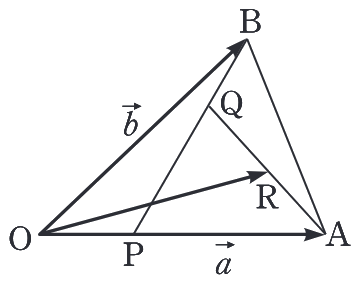
\includegraphics[width=\dmfigw]{figures/fig-176-359.png}\end{minipage}\par
